\documentclass{article}
\usepackage{amsmath}
\usepackage{upgreek}
\usepackage{dsfont}
\usepackage{mdframed}
%margin package
\usepackage[margin=1in,includefoot]{geometry}
%graphics packages
\usepackage{graphicx}
\usepackage{float}
%pseudocode packages
\usepackage{amsmath}
\usepackage{algorithm}
\usepackage[noend]{algpseudocode}
%hyperlinks
\usepackage{hyperref}

\begin{document}

\begin{titlepage}
	\begin{center}
	\line(1,0){400}\\
	\huge{\bfseries First report on the paper "Iterated Tabu Search and 		Variable Neighborhood Descend for packing unequal circles into a circular container".}\\
	\line(1,0){400}\\
	\textsc{\Large About the details of the paper, description of the algorithm and the reach of the final project}
	\end{center}
	\vspace{5in}
	\begin{flushright}
	\textsc{\large Author: Wilbert Pumacay\\}
	June 30, 2017
	\end{flushright}
	
\end{titlepage}

\section{Description of the problem}\label{sec:intro}%%%%%%%%%%%%%%%%%%%%%%%%%%%%%%%%%%%%%%%%%%%%%%%%%%%%%%%%%%%%
%% Brief description of the problem %%%%%%%%%%%%%%%%%%%
The problem to be studied is the circle packing problem, which consists of finding the minimum radius $R$ of a circle container that encloses a given set of $n$ circles such that none of them overlaps with each other nor the container. This is formally formulated as follows:\\
%%%%%%%%%%%%%%%%%%%%%%%%%%%%%%%%%%%%%%%%%%%%%%%%%%%%%%%

%% MATHEMATICAL PROBLEM FORMULATION %%%%%%%%%%%%%%
Given a circle container $D_{0}$ of variable radius $R$, as well as n circles with known radius $r_{1},r_{2},\hdots,r_{n}$. Let $D_{0}.center=(0,0)$ and $D_{i}.center=(x_{i},y_{i}) \forall i = 1,\hdots,n$. Find a solution 
$[R,\lbrace(x_{1},y_{1}),\hdots,(x_{n},y_{n})\rbrace]=[R,X]$ with minimum $R$ such that the configuration is feasible (no overlaps), which can be expressed mathematically as follows:
\begin{gather*}
R - r_{i} \geq d_{i} = \sqrt{x^{2}_{i} + y^{2}_{i}}, \forall i=1,\hdots,n \\
r_{i} + r_{j} \geq d_{ij} = \sqrt{(x_{i}-x_{j})^{2} + (y_{i}-y_{j})^{2}}, \forall i \neq j \textit{ in } 
\lbrace1,\hdots,n\rbrace \\
\end{gather*}

The configurations that do not satisfy the constraints are called infeasible. This can be measured using the potential function $U=\sum\limits_{i=0}^{n-1}\sum\limits_{j=i+1}^{n}\frac{1}{2}O_{ij}^{2}$ which measures the amount of overlap between all circles $D_{0},\hdots,D_{n}$.\\
%%%%%%%%%%%%%%%%%%%%%%%%%%%%%%%%%%%%%%%%%%%%%%%%%%

%% some figures %%%%%%%%%%%%%
The following figures show some examples of feasible and unfeasible solutions. Figure 1 shows a case of a feasable packing for the equal circle packing problem ( PECC ), and Figure 2 shows an example of an infeasible solution for the unequal circle packing problem ( PUCC ), which is the one the paper is focused on.

%% fig1 optimal solution for pecc
\begin{figure}[H]
	\centering
	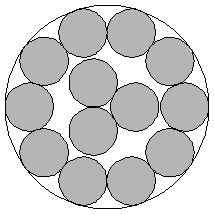
\includegraphics[scale=0.4]{/home/gw/Documents/wilbert/cs_master/courses/term1/datastructures_and_algorithms/cppfiddle/latex/imgs/pecc.jpg}
	\caption{A feasible configuration for the PECC problem}
	\label{fig:img_pecc}
\end{figure}

%% fig2 infeasible solution for pucc
\begin{figure}[H]
	\centering
	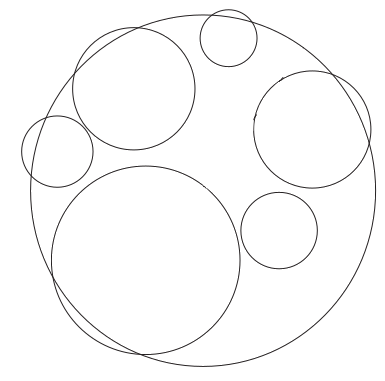
\includegraphics[scale=0.25]{/home/gw/Documents/wilbert/cs_master/courses/term1/datastructures_and_algorithms/cppfiddle/latex/imgs/img_pucc_infeasible.png}
	\caption{An infeasible configuration for the PUCC problem}
	\label{fig:img_pecc}
\end{figure}

%%%%%%%%%%%%%%%%%%%%%%%%%%%%%

%% ending section %%%%%%%%%%%
This packing problem is essentially NP-Hard, so the optimal solutions can't be achieved by an algorithm. That is why the approach taken is to get approximate solutions by using metaheuristics, method that will be discussed in the following sections.\\
%%%%%%%%%%%%%%%%%%%%%%%%%%%%%

%%%%%%%%%%%%%%%%%%%%%%%%%%%%%%%%%%%%%%%%%%%%%%%%%%%%%%%%%%%%%%%%%%%%%%%%%%%%%%%%%%%%%%%%%%%%%%%%%%%%%%%%%%%%%%%%%


\section{Description of the solution and the metaheuristic(s) used}\label{sec:solution}%%%%%%%%%%%%%%%%%%%%%%%%%%
%% Brief description of the solution %%%%%%%%%%%%%%%%%%
The solution method falls into the category of optimization methods. The solution is improved iteratively using an optimizer and a combination of two metaheuristics. The authors' solution starts with a configuration $(R,X)$ of container radius and circle centers, and in each iteration they improve the configuration by reducing the radius of the container ( an optimizer is used in this step ) and reorganizing ( metaheuristics used here for local search ) the configuration in such a way that the container's radius is smaller each time and the configuration $(R,X)$ is feasible. This process can be seen in Figure 3 and Figure 4.\\

%% fig3 optimization step
\begin{figure}[H]
	\centering
	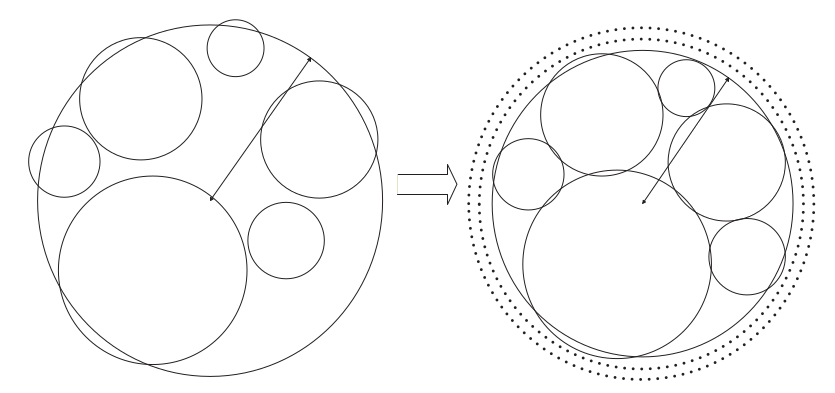
\includegraphics[scale=0.3]{/home/gw/Documents/wilbert/cs_master/courses/term1/datastructures_and_algorithms/cppfiddle/latex/imgs/img_optimization_step.png}
	\caption{Reduction of the container radius in the optimization step.}
	\label{fig:img_pecc}
\end{figure}

%% fig4 intensification step
\begin{figure}[H]
	\centering
	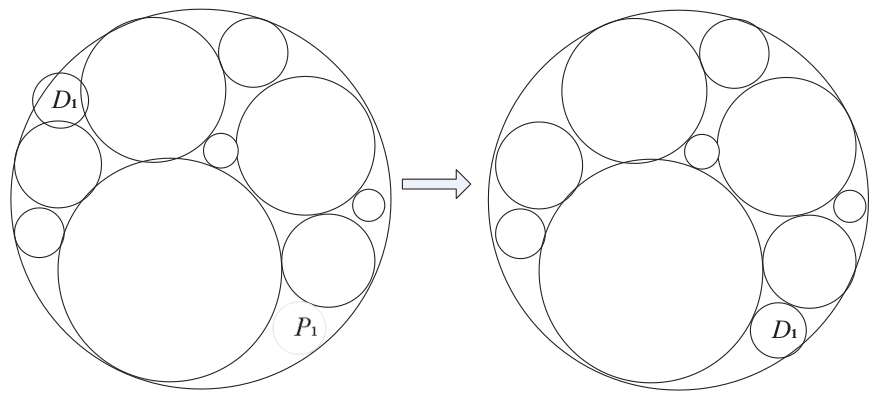
\includegraphics[scale=0.3]{/home/gw/Documents/wilbert/cs_master/courses/term1/datastructures_and_algorithms/cppfiddle/latex/imgs/img_intensification_step.png}
	\caption{Reorganization of the circles in the intensification step.}
	\label{fig:img_pecc}
\end{figure}
%%%%%%%%%%%%%%%%%%%%%%%%%%%%%%%%%%%%%%%%%%%%%%%%%%%%%%%

%% Description of the steps involved in the solution %%
The proposed solution is divided in a heirarchical way, which performs the method mentioned earlier in three phases. These phases are described as follows:

\begin{itemize}
\item Continuous Optimization : In this phase a numerical optimization method is used to reduce the container radius and centers configuration, which will be used in a later phase of the solution.
\item Intensification : Here, two metaheuristics are used, namely \textbf{Tabu Search} and \textbf{Variable Neighborhood Descend} to adjust the solutions from the previous phase by exploring two neighborhoods: \textit{Swap} and \textit{Insert}, which consists of variations to explore by swaping circles centers and inserting one circle into a vacant space respectively.
\item Diversification : In this pase the solutions are perturbed according to a random reset strategy to diversify the exploration of the previous step.
\end{itemize}

%%%%%%%%%%%%%%%%%%%%%%%%%%%%%%%%%%%%%%%%%%%%%%%%%%%%%%%

%% Pseudocode of the solution %%%%%%%%%%%%%%%%%%%%%%%%%
The solution described is expressed in the following pseudocode :\\

\begin{algorithm}
\caption{Three-step heirarchical solution}\label{solution_pseudocode}
\begin{algorithmic}[1]
\State $\textit{Set initial configuration }(R,X)$
\While{$\textit{(Stop criterion)}$}
	\State $(R,X)=\textit{PerturbationStep}((R,X))$
	\State $(R,X)=\textit{IntensificationStep}((R,X))$
	\State $(R,X)=\textit{OptimizationStep}((R,X))$
\EndWhile
\Return $(R,X)$
\end{algorithmic}
\end{algorithm}

%%%%%%%%%%%%%%%%%%%%%%%%%%%%%%%%%%%%%%%%%%%%%%%%%%%%%%%


%% Description of the metaheuristics used %%%%%%%%%%%%%
The metaheuristics used in the solution are \textit{Tabu Search}(TS) and \textit{Variable Neighborhood Descend}(VND), which are used in the second phase of the solution ( intensification phase ).

\begin{itemize}
\item \textbf{Tabu Search :} As described in the references used by the authors, Tabu search works with a neighborhood, which in this case is the \textit{Swap Neighborhood}( SN ) described earlier. Once a swap is taken based on the neighborhood, it is marked as Tabu for $\delta$ iterations.
\item \textbf{Variable Neighborhood Descend :} Here, the basic version of Variable Neighborhood Search (VNS) is used. For the local search part of the VND the swap neighborhood is used. Then, the insert neighborhood is used in the varying part of the VND routine to look for better solutions.
\end{itemize}

%%%%%%%%%%%%%%%%%%%%%%%%%%%%%%%%%%%%%%%%%%%%%%%%%%%%%%%

\section{Description of the algorithms}\label{sec:algorithms}%%%%%%%%%%%%%%%%%%%%%%%%%%%%%%%%%%%%%%%%%%%%%%%%%%%%

%% Intro %%%%%%%%%%%%
As described earlier, the algorithm is divided into 3 phases.
%%%%%%%%%%%%%%%%%%%%%

\begin{itemize}
\item[a)] \textbf{Continuous optimization using the LBFGS method.}\\
This is the part in charge of reducing the radius of the container and getting the circles closer to each other. The method used is a variant of the LBFGS method. LBFGS stands for "Limited-memory Broyden-Fletcher-Goldfarb-Shanno", which is a quasi-Newton method, kind of similar to gradient descent (it uses an approximation of the gradient, or Hessian matrix instead of a Jacobian). Here, the function we are going to be taking the Hessian of is our potential function $U$ described in the first section. The variant used is called BS-LBFGS, which adds a \textit{Binary Search} step (BS) to the LBFGS method.

\item[b)] \textbf{Intensification using TS and VND metaheuristics.}\\
In this phase, two neighborhoods are created as described earlier ( Swap and Insert neighborhoods). This phase is basically a search that exploits this two neighborhoods using the metaheuristics already described.

\item[c)] \textbf{Diversification using a Random Reset Perturbation strategy.}\\
This phase involves perturbating some circles ( the quantity is called \textit{perturbation strength}) around the container by applying a perturbation strategy described in the references. The result of this phase is that the solutions of the previous search phase are diversified, allowing to explore other promising regions of the search space.

\end{itemize}

%%%%%%%%%%%%%%%%%%%%%%%%%%%%%%%%%%%%%%%%%%%%%%%%%%%%%%%%%%%%%%%%%%%%%%%%%%%%%%%%%%%%%%%%%%%%%%%%%%%%%%%%%%%%%%%%%

\section{Description of the instances and algorithms to be implemented}\label{sec:algorithms}%%%%%%%%%%%%%%%%%%%%

%% About the instances %%%%%%%%%%%%

The instances used in the paper come from a contest host in this \href{http://www.packomania.com/}{site}, and a benchmark proposed in this \href{http://www.sciencedirect.com/science/article/pii/S0305054805000031?via}{paper}. 
The contest benchmarks are a set $\lbrace (n,results) \rbrace$ for two types of circles' radius definitions: $r_{i}=i$ and $r_{i}=i^{-1/2}$. The second benchmark is a table proposed in the mentioned paper (Figure 5).\\

%% fig5 NR benchmark
\begin{figure}[H]
	\centering
	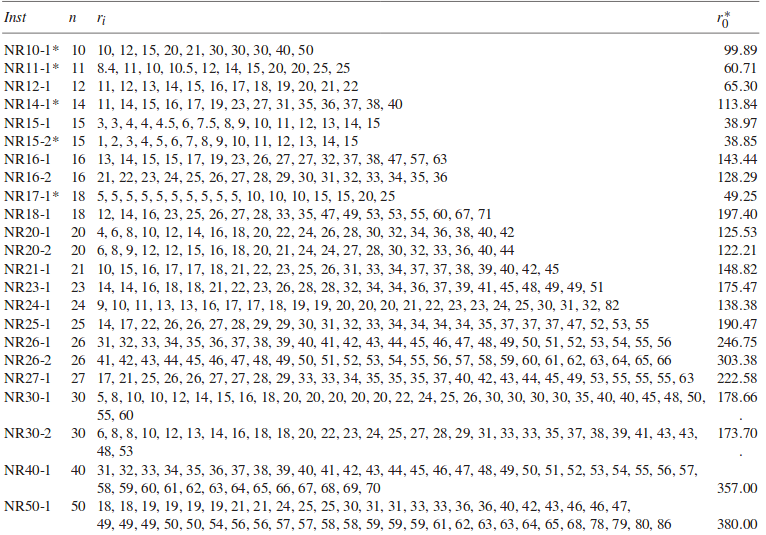
\includegraphics[scale=0.4]{/home/gw/Documents/wilbert/cs_master/courses/term1/datastructures_and_algorithms/cppfiddle/latex/imgs/img_nr_benchmark.png}
	\caption{NR benchmark.}
	\label{fig:img_pecc}
\end{figure}

%%%%%%%%%%%%%%%%%%%%%%%%%%%%%%%%%%%

%% About what is going to be implemented %%%
The parts that are going to be implemented are all the necessary modules for the ITS-VND algorithm proposed, which include the optimization using BS-LBFGS, the metaheuristics (TS and VND) in the intensification phase, and the perturbation strategy in the diversification phase. The diagram showns in Figure 6 show the modules that are going to be implemented.\\

%%%%%%%%%%%%%%%%%%%%%%%%%%%%%%%%%%%%%%%%%%%%

%% fig6 modules to be programmed
\begin{figure}[H]
	\centering
	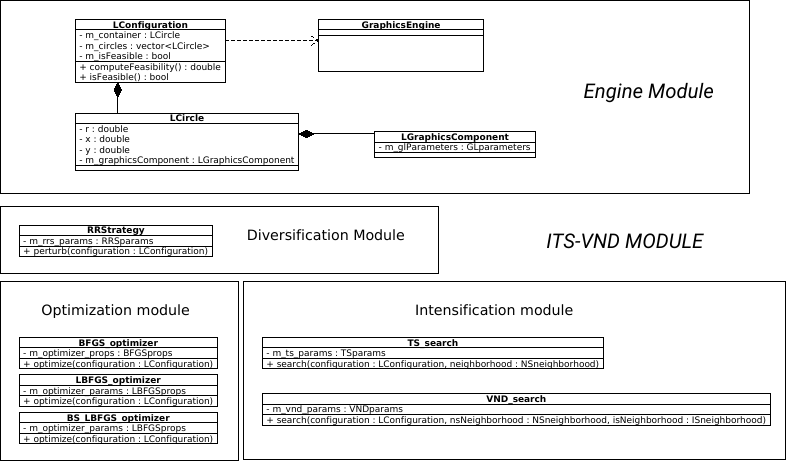
\includegraphics[scale=0.75]{/home/gw/Documents/wilbert/cs_master/courses/term1/datastructures_and_algorithms/cppfiddle/latex/imgs/img_modules.png}
	\caption{Modules to be implemented.}
	\label{fig:img_pecc}
\end{figure}

%%%%%%%%%%%%%%%%%%%%%%%%%%%%%%%%%%%%%%%%%%%%%%%%%%%%%%%%%%%%%%%%%%%%%%%%%%%%%%%%%%%%%%%%%%%%%%%%%%%%%%%%%%%%%%%%%
\end{document}